\id{МРНТИ 65.63.33}

{\bfseries ФУНКЦИОНАЛДЫҚ БАҒЫТТАҒЫ ӨСІМДІК СУСЫНДАРЫНЫҢ ОРГАНОЛЕПТИКАЛЫҚ
КӨРСЕТКІШТЕРІ}

{\bfseries Н.E. Альжаксина}
\begin{figure}[H]
	\centering
	
\includegraphics[width=0.8\textwidth]{media/pish2/image5}
	\caption*{}
\end{figure}

\textbackslash{} {\bfseries \textsuperscript{\envelope }, М.С.
\begin{figure}[H]
	\centering
	
\includegraphics[width=0.8\textwidth]{media/pish2/image5}
	\caption*{}
\end{figure}

И.Е.
\begin{figure}[H]
	\centering
	
\includegraphics[width=0.8\textwidth]{media/pish2/image5}
	\caption*{}
\end{figure}


\emph{Астана филиалы ЖШС «Қазақ қайта өңдеу және тағам өнеркәсіптері
ғылыми-зерттеу}

\emph{институты, Астана, Қазақстан}

{\bfseries \textsuperscript{\envelope }}Корреспондент-автор:
\href{mailto:alzhaxina@inbox.ru}{\nolinkurl{alzhaxina@inbox.ru}}

Ғылыми зерттеудің мақсаты - функционалды өсімдік негізіндегі сусындардың
оңтайлы органолептикалық сипаттамаларын анықтау. Сүт-жаңғақ,
сүт-дәнді-дақыл және сүт-дәнді-бұршақ жүйелер негізінде өсімдік
сусындарын өндіруге арналған компоненттерді таңдау жаңғақтарда,
дәнді-дақылдарда және бұршақ тұқымдастарында ақуыз, липидтер және
тағамдық талшықтардың құрамына байланысты жүргізілді. Зерттеу барысында
рецептуралар әзірленіп, сыналып, әртүрлі өсімдік сусындарының үлгілері
дайындалып, дәмдік бағалаудан өтті. Зерттелген композициялар МемСТ
талаптарына толық сәйкес келетін жоғары органолептикалық көрсеткіштерге
ие болды. Функционалды сусын үлгілерін органолептикалық әдіспен
зерттеді. Сусындардың дәмдік сипаттамаларын бағалау үшін жетілдірілген
бес балдық органолептикалық бағалау шкаласы қолданылды. Органолептикалық
бағалау келесі көрсеткіштер бойынша жүргізілді: сыртқы түрі, түсі, хош
иісі, дәмі және консистенциясы. Жергілікті өсімдік шикізатын, сондай-ақ
өсімдік негізіндегі сусындарды өндіруде тұрақтандырғыштар мен табиғи
тәттілендіргіштерді, әсіресе гуар камеді, ксантан камеді және ваниль
сығындысы қолдану жоғары органолептикалық қасиеттері бар жаңа өсімдік
сусындарының ассортиментін жасауға мүмкіндік береді. Зерттеу нәтижесінде
№1 үлгінің - жаңғақ жемісі, су және гуар камедінің (1:1:1 қатынасында)
қоспасы - ең жоғары профилограмма көлеміне ие екені анықталды.

{\bfseries Түйін сөздер:} органолептикалық көрсеткіштер, өсімдік сусындары,
функционалдық бағыт, сүт-жаңғақ жүйесі, сүт-дәнді дақыл жүйесі,
сүт-дәнді-бұршақ жүйесі, сыртқы түрі, консистенция.

{\bfseries ОРГАНОЛЕПТИЧЕСКИЕ ПОКАЗАТЕЛИ РАСТИТЕЛЬНЫХ НАПИТКОВ
ФУНКЦИОНАЛЬНОЙ НАПРАВЛЕННОСТИ}

{\bfseries Н.E. Альжаксина\textsuperscript{\envelope }, М.С. Мантай, И.Е.
Аубакирова}

\emph{Астанинский филиал ТОО «Казахский научно-исследовательский
институт перерабатывающей и пищевой промышленности», Астана, Казахстан,}

\emph{е-mail:
\href{mailto:alzhaxina@inbox.ru}{\nolinkurl{alzhaxina@inbox.ru}}}

Цель научного исследования - определение оптимальных органолептических
характеристик растительных напитков функциональной направленности.
Подбор компонентов для получения растительных напитков на основе
молочно-ореховых, молочно-злаковых и молочно-зернобобовых систем в
рецептурах проводился в зависимости от содержания белка, липидов,
пищевых волокон в грецких орехах, злаках и бобах. В ходе исследований
разработаны, апробированы рецептуры, изготовлены и продегустированы
образцы различных композиций растительных напитков. У исследуемых
композиций хорошие органолептические показатели, соответствующие всем
предъявляемым требованиям ГОСТ. Изготовленные образцы функциональных
напитков исследовали органолептическим методом. Для оценки вкусовых
характеристик напитков применяли модернизированную пятибалльную шкалу
органолептической оценки. Органолептическую оценку напитков принято
проводить по следующим показателям: внешний вид, цвет, аромат, вкус и
консистенция. Использование местного растительного сырья, а также
стабилизаторов и природных подсластителей, в частности гуаровая камедь,
ксантановая камедь и ванильный экстракт для производства растительных
напитков на основе плодов ореха, злаковых и зернобобовых культур, дает
возможность получения нового ассортимента растительных напитков с
высокими органолептическими показателями. В результате проведенных
исследований установлено, что наибольший объем занимает профилограмма
образца №1 - смесь плодов ореха, воды и гуаровая камедь (соотношение
1:1:1).

{\bfseries Ключевые слова:} органолептические показатели, растительные
напитки, функциональная направленности, молочно-ореховая,
молочно-злаковая и молочно-зернобобовая системы, внешний вид,
консистенция.

{\bfseries ORGANOLEPTIC CHARACTERISTICS OF FUNCTIONAL HERBAL DRINKS}

{\bfseries N. Alzhaxina\textsuperscript{\envelope }, М. Mantai, I. Aubakirova,}

\emph{Astana branch «Kazakh research institute of processing and food
industry» LTD, Astana, Kazakhstan,}

\emph{е-mail:
\href{mailto:alzhaxina@inbox.ru}{\nolinkurl{alzhaxina@inbox.ru}}}

The aim of this scientific research is to determine the optimal
organoleptic characteristics of functional plant-based beverages. The
selection of components for the production of plant-based beverages
based on milk-nut, milk-cereal, and milk-legume systems was carried out
depending on the protein, lipid, and dietary fiber content in walnuts,
cereals, and legumes. During the study, formulations were developed and
tested, and samples of various plant-based beverage compositions were
produced and evaluated. The tested compositions demonstrated good
organoleptic properties that meet all the requirements of GOST
standards. The functional beverage samples were assessed using the
organoleptic method. A modified five-point organoleptic evaluation scale
was used to assess the taste characteristics of the beverages.
Organoleptic evaluation was conducted based on the following criteria:
appearance, color, aroma, taste, and consistency. The use of locally
sourced plant raw materials, as well as stabilizers and natural
sweeteners - such as guar gum, xanthan gum, and vanilla extract - in the
production of plant-based beverages based on nuts, cereals, and legumes
allows for the development of a new range of plant-based beverages with
high organoleptic properties. As a result of the research, it was found
that Sample No. 1 - comprising a mixture of walnut, water, and guar gum
(in a 1:1:1 ratio) - had the highest profile volume.

{\bfseries Keywords:} organoleptic parameters, plant-based beverages,
functional purpose, milk-nut, milk-cereal, and milk-legume systems,
appearance, texture.

{\bfseries Кіріспе.} Қазіргі өмір салтының қарқыны соңғы онжылдықтарда
едәуір жеделдеп, заманауи адамды тұрақты интеллектуалдық және
эмоционалдық күйзеліс жағдайына қояды. Бұл жалпы физикалық жағдай мен
халықтың әртүрлі әлеуметтік топтарының денсаулығына кері әсер етеді.
Толыққанды және теңгерімді тамақтанудың болмауы, жаңа тағам дайындауға
уақыттың жетіспеуі, сондай-ақ қажетті микро және макронутриенттердің
тапшылығы бүгінде ел тұрғындарының көпшілігіне тән жағдайға айналды
{[}1, 2{]}. Осындай жағдайда дайын, қолжетімді әрі қоректік өнімдер
қажеттілікке айналады. Функционалдық қасиеттері бар сергіткіш сусындар
-- қазіргі жұмыскер адамның талаптарына толық сәйкес келетін өнім
топтарының бірі. Бұл сусындар адам ағзасын қажетті сұйықтықпен
қамтамасыз етіп қана қоймай, құрамындағы биологиялық белсенді заттар
арқылы кең таралған аурулардың дамуын болдырмауға, сондай-ақ қоршаған
ортаның қолайсыз факторларынан қорғауға мүмкіндік береді {[}3-6{]}.

Қазіргі адамның рационы құрамына қарай әртүрлі әрі күрделі тағам
өнімдерінен тұрады. Осыған байланысты азық-түлік индустриясының жаңа
бағыты -- өсімдік сүтін өндіру дами бастады. Алғашқы өсімдік сусыны
ретінде дәстүрлі сиыр сүтіне пайдалы балама ретінде соя сүті жасалды.
Соңғы жылдары дәнді, бұршақты дақылдар мен жаңғақтардың функционалдық
қасиеттерін зерттеуге және оларды жаңа өсімдік сусындарын жасау үшін
қолдануға ерекше назар аударылуда {[}7{]}.

Соңғы жылдары функционалдық мақсаттағы өсімдік сусындары кеңінен танымал
болды. Олар -- жаңғақ, бұршақ және дәнді дақылдар мен өсімдік тектес
әртүрлі заттардан жасалған түрлі композициялар. Бұл сусындардың ерекше
артықшылығы -- олардың құрамында дәрумендер, макро- және
микроэлементтер, тағамдық талшықтардың болуы. Мұндай сусындарды өндіруде
тек табиғи өсімдік шикізатын, химиялық қоспаларсыз қолдану қажет.

Өсімдік сусындарының органолептикалық бағасы келесі көрсеткіштер бойынша
жүргізіледі: сыртқы түрі, хош иісі, түсі, дәмі және консистенциясы
{[}8{]}.

{\bfseries Материалдар мен әдістер.} Зерттеудің объектілері ретінде дәнді
(арпа), дәнді-бұршақты (маш) және жаңғақ (грек жаңғағы) негізіндегі
өсімдік сусындары таңдалды. Әлсіз айқындалған дәмдік және хош иістік
қасиеттерге байланысты бұл сусындардың үйлесімділігін арттыру үшін
оларды тұрақтандырғыштар мен тәттілендіргіштер қосып араластырды.
Зерттелген өсімдік сусындарының органолептикалық бағалау шкаласы МемСТ
35075-2024 «Өсімдік негізіндегі сусындар» талаптарына сәйкес жасалды.
Табиғи өсімдік шикізатынан алынған ингредиенттердің оңтайлы қатынасын
анықтау кезінде дайын сусындардың органолептикалық көрсеткіштері негізгі
критерий ретінде таңдалды. Өсімдік сусындарының органолептикалық бағасы
-- бұл өнімнің сапасының ең маңызды көрсеткіші, өйткені ол
тұтынушылардың сұранысын анықтап, өнімді нарықта ілгерілетуге ықпал
етеді. Ингредиенттердің әртүрлі вариацияларымен 9 модельдік сусынның
рецептурасы жасалды.

{\bfseries Нәтижелер және талқылау.~} Органолептикалық зерттеулер
дегустациялық әдіске сәйкес, АФ ЖШС «ҚҚӨжТӨҒЗИ» зертханасының
қызметкерлерінен құралған дегустациялық комиссия тарапынан жүргізілді.
Зерттеулер МемСТ 6687.5-86 және МемСТ 8756.11-2015 талаптарына сәйкес
жүзеге асырылды.

Алынған өсімдік сусындарының органолептикалық бағалау сипаттамалық
шкаласы 1-кестеде берілген.

{\bfseries 1 - кесте. Зерттелетін өсімдік сусындарының үлгілерін
органолептикалық бағалаудың сипаттамалық шкаласы~}

% \begin{longtable}[]{@{}
%   >{\raggedright\arraybackslash}p{(\columnwidth - 2\tabcolsep) * \real{0.0739}}
%   >{\raggedright\arraybackslash}p{(\columnwidth - 2\tabcolsep) * \real{0.9261}}@{}}
% \toprule\noalign{}
% \begin{minipage}[b]{\linewidth}\raggedright
% Балл
% \end{minipage} & \begin{minipage}[b]{\linewidth}\raggedright
% Сусынның органолептикалық бағалауының сипаттамасы
% \end{minipage} \\
% \midrule\noalign{}
% \endhead
% \bottomrule\noalign{}
% \endlastfoot
% 5 & Біртекті, мөлдір емес, лайлы сұйықтық. Бөгде қосындыларсыз. Қою
% консистенцияға жол беріледі. Сақтау кезінде қабаттану мүмкін, бірақ
% шайқаған кезде құрылымы қалпына келеді. Табиғи тұнба, қалқымалар,
% түйіршіктер біркелкі таралған, сусынның қабылдануына әсер етпейді. Беткі
% қабатында жұқа майлы үлдір пайда болуы мүмкін.
% 
% Түсі -- ақ, кілегейлі, сарғыш немесе жасылдау реңкті, не болмаса шикізат
% түріне байланысты ашық сұр. Масса бойынша біркелкі. Қосылған
% ингредиенттерге байланысты түстің өзгеруі мүмкін. Сақтау кезінде шамалы
% түс біркелкісіздігі байқалуы мүмкін.
% 
% Дәмі мен иісі -- айқын, үйлесімді, қолданылған шикізат пен тағамдық
% ингредиенттерге толық сәйкес келеді. Жеңіл ұнтақтық сезілуі мүмкін,
% бірақ сусын сапасына әсер етпейді. Бөгде дәм мен иіс жоқ. \\
% 4 & \begin{minipage}[t]{\linewidth}\raggedright
% Біртекті, лайлы сұйықтық, тығыздығы мен тұтқырлығы аздап өзгеруі
% мүмкін.\\
% Табиғи шыққан ұсақ ұйынды немесе тұнба пайда болуы ықтимал, бірақ олар
% сыртқы көріністі нашарлатпайды. Майлы үлдір өте әлсіз байқалады.
% 
% Түсі -- табиғи, белгіленген ауқымға сәйкес келеді, бірақ аздап біркелкі
% емес рең байқалуы мүмкін. Сақтау кезінде түсінің шамалы өзгеруі мүмкін.
% 
% Дәмі мен иісі -- шикізатқа сәйкес, бірақ айқын емес. Жеңіл ұнтақтық
% сезілуі мүмкін, бірақ жалпы қабылдауға кедергі келтірмейді. Бөгде иіс
% пен дәм жоқ.\strut
% \end{minipage} \\
% 3 & \begin{minipage}[t]{\linewidth}\raggedright
% Біртектілігінің аздаған өзгерістері: айқын қабаттану, орташа мөлшерде
% қалқымалар немесе түйіршіктер.\\
% Тұнба айқын байқалады, бірақ шайқаған кезде жартылай таралады.
% Консистенциясы күтілгеннен сұйықтау.
% 
% Түсі -- рұқсат етілген шектерде, бірақ біркелкі емес. Әсіресе сақтау
% кезінде әртүрлі түстегі аймақтар пайда болуы мүмкін.
% 
% Дәмі мен иісі -- әлсіз, типтік дәмдік профилінен сәл ауытқуы мүмкін.
% Жеңіл ұнтақтық анық сезіледі. Бөгде реңктер болуы мүмкін, бірақ сусынның
% қабылдануына айтарлықтай әсер етпейді.\strut
% \end{minipage} \\
% 2 & \begin{minipage}[t]{\linewidth}\raggedright
% Айқын қабаттану, тығыз тұнба, шайқаған кезде таралмайды.\\
% Қалқымалар мен түйіршіктердің көп мөлшері сусынның қабылдануын
% нашарлатады. Майлы үлдір қалың әрі анық байқалады.
% 
% Түсі -- біркелкі емес, айқын түсті аймақтар байқалады. Сыртқы көріністі
% нашарлататын бөгде реңктер болуы мүмкін.
% 
% Дәмі мен иісі -- әлсіз, күңгірт, бөгде реңктер байқалады. Айқын ұнтақтық
% немесе кедір-бұдыр сезіледі. Бөгде иіс пен дәм байқалады, бірақ өткір
% емес.\strut
% \end{minipage} \\
% 1 & \begin{minipage}[t]{\linewidth}\raggedright
% Біртекті емес, тым сұйық немесе шамадан тыс қою консистенция.\\
% Күшті қабаттану, шайқағанда араласпайтын тығыз тұнба. Көптеген бөгде
% қосындылар, қалың және табиғи емес үлдір байқалады.
% 
% Түсі -- белгіленген ауқымға сәйкес келмейді. Айқын біркелкісіздік,
% сапаның бұзылғанын көрсететін бөгде реңктер бар.
% 
% Дәмі мен иісі -- шикізатқа сәйкес келмейді, бөгде иіс пен дәм айқын
% сезіледі. Айқын ұнтақтық, жағымсыз құрылым байқалады.\strut
% \end{minipage} \\
% \end{longtable}

Сусындардың дәмдік қасиеттерін бағалау үшін жетілдірілген бес балдық
органолептикалық бағалау шкаласы қолданылды {[}9{]}. Сүт-жаңғақ,
сүт-дақыл және сүт-дәнді-бұршақ жүйелері негізіндегі өсімдік
сусындарының дегустациялық бағалау нәтижелері 2-кестеде көрсетілген.

{\bfseries 2 - кесте. Өсімдік сусындары үлгілерінің органолептикалық
көрсеткіштері}

% \begin{longtable}[]{@{}
%   >{\raggedright\arraybackslash}p{(\columnwidth - 4\tabcolsep) * \real{0.0977}}
%   >{\raggedright\arraybackslash}p{(\columnwidth - 4\tabcolsep) * \real{0.6629}}
%   >{\raggedright\arraybackslash}p{(\columnwidth - 4\tabcolsep) * \real{0.2394}}@{}}
% \toprule\noalign{}
% \begin{minipage}[b]{\linewidth}\raggedright
% Үлгі №
% \end{minipage} & \begin{minipage}[b]{\linewidth}\raggedright
% Сусындардың атауы
% \end{minipage} & \begin{minipage}[b]{\linewidth}\raggedright
% Балл
% \end{minipage} \\
% \midrule\noalign{}
% \endhead
% \bottomrule\noalign{}
% \endlastfoot
% \multicolumn{3}{@{}>{\raggedright\arraybackslash}p{(\columnwidth - 4\tabcolsep) * \real{1.0000} + 4\tabcolsep}@{}}{%
% Сүт-жаңғақ жүйесі} \\
% 1 & Жаңғақ жемістері -- су -- гуар камеді (1:1:1) & 4,8 \\
% 2 & Жаңғақ жемістері -- су -- каррагинан (2:1:1) & 4,7 \\
% 3 & Жаңғақ жемістері -- су -- лимон қышқылы (3:1:1) & 4,5 \\
% \multicolumn{3}{@{}>{\raggedright\arraybackslash}p{(\columnwidth - 4\tabcolsep) * \real{1.0000} + 4\tabcolsep}@{}}{%
% Сүт-дәнді-бұршақ жүйесі} \\
% 4 & Маш -- су -- гуаровая камеді (1:1:1) & 4,4 \\
% 5 & Маш -- су -- каррагинан (2:1:2) & 4,2 \\
% 6 & Маш -- су -- ваниль сығындысы (3:1:3) & 4,0 \\
% \multicolumn{3}{@{}>{\raggedright\arraybackslash}p{(\columnwidth - 4\tabcolsep) * \real{1.0000} + 4\tabcolsep}@{}}{%
% Сүт-дәнді дақыл жүйесі} \\
% 7 & Арпа -- су -- ксантан камеді (1:1:3) & 4,1 \\
% 8 & Арпа -- су -- каррагинан (2:1:2) & 4,2 \\
% 9 & Арпа -- су -- лецитин (3:1:2) & 4,0 \\
% \end{longtable}

2 - кестедегі органолептикалық бағалау нәтижелерін салыстыра отырып,
барлық үлгілердің сенсорлық сипаттамалар бойынша ұқсас екенін және
сапасы жоғары деңгейге жататынын атап өтуге болады. Барлық тоғыз үлгі
біркелкі консистенциямен сипатталады, бірақ кейбір үлгілер белгілі бір
уақыт өткеннен кейін екі фазаға бөлініп кетті. Бұл эмульсияның
тұрақсыздығын көрсетіп, өндіріс барысында эмульгаторлардың үлесін
арттыруды талап етеді. Бұл эмульсияны тұрақтандыруға және дайын өнімнің
тұтынушылық қасиеттерін сақтауға ықпал етеді. Жаңғақ жемістері бар
сусындар арасында ең жоғары дегустациялық бағаны 1, 2 және 3 үлгілері
алды. Олардың ұпайлары сәйкесінше жоғары болды. Гуар камеді және
каррагинан тұрақтандырғыштары бар сусындар арасында 1 және 2 үлгілеріне
ең жоғары баға - 4,7 балл берілді. Таңдалған үлгілер түс, дәм және хош
иіс бойынша үйлесімділікке ие, сондай-ақ ең жақсы органолептикалық
қасиеттерімен ерекшеленді. Зерттеулердің келесі кезеңі өсімдік
сусындарының оңтайлы рецептурасын әзірлеуге бағытталып, осы үлгілер
негізінде жүргізілді. Жергілікті шикізаттан алынған су мен жаңғақ, дәнді
және бұршақты дақылдардың оңтайлы қатынасын анықтау кезінде негізгі
критерий ретінде дайын өсімдік сусындарының органолептикалық
көрсеткіштері таңдалды. Тұрақтандырғыштар мен әртүрлі экстракттардың
шамадан тыс мөлшерде енгізілуі, әсіресе сүт-дақыл жүйесінде
байқалғандай, сусынның дәмін нашарлатып, органолептикалық бағалауға
теріс әсер етеді.

Алынған нәтижелердің математикалық өңдеуі профильдік әдіспен --
график-профилограмма құру арқылы жүргізілді. Бұл әдіс өнімнің
сипаттамалық белгілерін диаграмма осьтерінде көрсетуге негізделген.
Әрбір сипаттамалық белгінің қарқындылығы бес балдық шкала бойынша
осьтерде белгіленеді, ал осьтердегі нүктелерді қосу арқылы зерттелетін
өнімнің дәмдік профилі -- профилограмма құрылады. Графикте ең үлкен
көлемді қамтитын профилограмма оңтайлы болып есептеледі {[}10, 11{]}.

Сүт-жаңғақ, сүт-дақыл және сүт-дәнді-бұршақ жүйелері негізіндегі өсімдік
сусындарының зерттелген үлгілерін талдау нәтижелері 1-суретте
көрсетілген.

% \begin{longtable}[]{@{}
%   >{\raggedright\arraybackslash}p{(\columnwidth - 2\tabcolsep) * \real{0.5013}}
%   >{\raggedright\arraybackslash}p{(\columnwidth - 2\tabcolsep) * \real{0.4987}}@{}}
% \toprule\noalign{}
% \begin{minipage}[b]{\linewidth}\raggedright
% \begin{figure}[H]
% 	\centering
% 	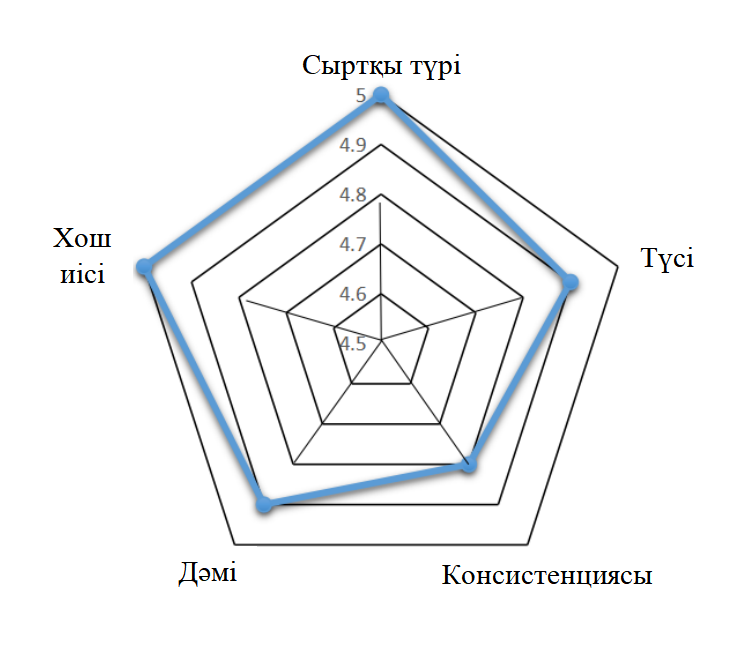
\includegraphics[width=0.8\textwidth]{media/pish2/image6}
% 	\caption*{}
% \end{figure}
% 
% \end{minipage} & \begin{minipage}[b]{\linewidth}\raggedright
% \begin{figure}[H]
% 	\centering
% 	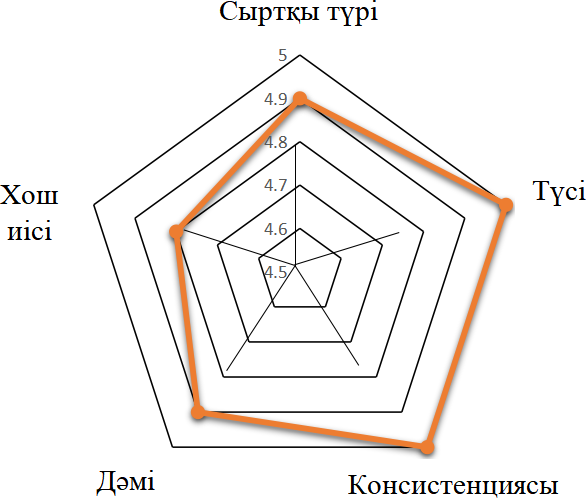
\includegraphics[width=0.8\textwidth]{media/pish2/image7}
% 	\caption*{}
% \end{figure}
% 
% \end{minipage} \\
% \midrule\noalign{}
% \endhead
% \bottomrule\noalign{}
% \endlastfoot
% Үлгі № 1 - Сүт-жаңғақ жүйесі & Үлгі № 4 - Сүт-дәнді-бұршақ жүйесі \\
% \multicolumn{2}{@{}>{\raggedright\arraybackslash}p{(\columnwidth - 2\tabcolsep) * \real{1.0000} + 2\tabcolsep}@{}}{%
% \begin{figure}[H]
% 	\centering
% 	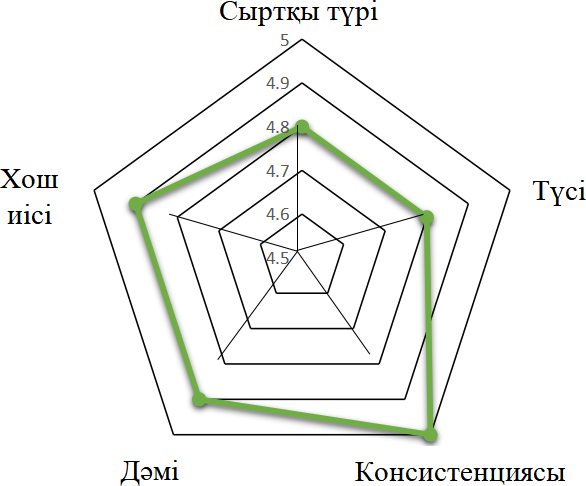
\includegraphics[width=0.8\textwidth]{media/pish2/image8}
% 	\caption*{}
% \end{figure}
% 
% \multicolumn{2}{@{}>{\raggedright\arraybackslash}p{(\columnwidth - 2\tabcolsep) * \real{1.0000} + 2\tabcolsep}@{}}{%
% Үлгі № 8 - Сүт-дәнді дақыл жүйесі} \\
% \end{longtable}

{\bfseries 1 - сурет. Өсімдік негізіндегі сусынның профилограммасы}

1-суретте №1 үлгінің профилограммасының ең үлкен көлемді алатыны анық
көрінеді. Осыған байланысты, одан әрі зерттеуге дәл осы нұсқа таңдалды.
Бұл үлгінің рецептурасына жаңғақ жемістері, су және гуар камеді 1:1:1
қатынасында кірді.

Өсімдік сусындарына арналған шикізат шығындарының нормалары 3-кестеде
көрсетілген.

{\bfseries 3 - кесте. Өсімдік сусындарының шикізат шығындарының нормалары}

% \begin{longtable}[]{@{}
%   >{\raggedright\arraybackslash}p{(\columnwidth - 2\tabcolsep) * \real{0.4878}}
%   >{\raggedright\arraybackslash}p{(\columnwidth - 2\tabcolsep) * \real{0.5122}}@{}}
% \toprule\noalign{}
% \begin{minipage}[b]{\linewidth}\raggedright
% Шикізат атауы, \%
% \end{minipage} & \begin{minipage}[b]{\linewidth}\raggedright
% Дайын сусынның құрамындағы шикізат (мл)
% \end{minipage} \\
% \midrule\noalign{}
% \endhead
% \bottomrule\noalign{}
% \endlastfoot
% \multicolumn{2}{@{}>{\raggedright\arraybackslash}p{(\columnwidth - 2\tabcolsep) * \real{1.0000} + 2\tabcolsep}@{}}{%
% Сүт-жаңғақ жүйесі} \\
% Грек жаңғағы 15,7\% & 39.25 \\
% Су & 209 \\
% Гуар камеді 0,15\% & 0.38 \\
% Ксантан камеді 0,15\% & 0.38 \\
% Тұз & 0.25 \\
% Ваниль сығындысы 0,28\% & 0.7 \\
% \multicolumn{2}{@{}>{\raggedright\arraybackslash}p{(\columnwidth - 2\tabcolsep) * \real{1.0000} + 2\tabcolsep}@{}}{%
% Сүт-дәнді дақыл жүйесі} \\
% Арпа 10\% & 25 \\
% Су & 218 \\
% Тұз & 0.25-0.5 \\
% Сахароза / глюкоза 1--1.5\% & 2.5-3.75 \\
% Өсімдік майы 1\% & 2.5 \\
% Лецитин 0.03--0.05\% & 0.075-0.125 \\
% Ксантан камеді 0.02\% & 0.05 \\
% Гуар камеді 0.015\% & 0.037 \\
% Каррагинан 0.005--0.01\% & 0.0125-0.025 \\
% \multicolumn{2}{@{}>{\raggedright\arraybackslash}p{(\columnwidth - 2\tabcolsep) * \real{1.0000} + 2\tabcolsep}@{}}{%
% Сүт-дәнді-бұршақ жүйесі} \\
% Маш 18,2\% & 45.5 \\
% Су & 202 \\
% Тұз & 0.25-0.5 \\
% Ваниль сығындысы 0,28\% & 0.7 мл \\
% Гуар камеді 0,25\% & 0.62 \\
% \end{longtable}

{\bfseries Қорытынды.} Өсімдік негізіндегі сусындардың үлгілерін таңдау
ғылыми түрде негізделді, олар сүт-жаңғақ, сүт-дәнді-дақыл және сүт-
дәнді-бұршақ жүйелеріне негізделген. Дегустациялық бағалау нәтижесінде
1, 2 және 3-нөмірлі үлгілер ерекшеленді. 1 және 2-нөмірлі үлгілер
құрамына енгізілген тұрақтандырғыштардың арқасында 4,7 балл алды.
Оптималды нұсқа таңдалып, оның құрамына жаңғақ жемістері, су және гуар
камеді 1:1:1 арақатынасында енгізілді. Бұл компоненттер түсі, дәмі және
хош иісі бойынша жақсы үйлесім тауып, ең жоғары органолептикалық
қасиеттерге ие болды. Бұл эмульгаторлар мөлшерінің артуы нәтижесінде
эмульсияның тұрақтануын көрсетеді. Таңдалған өсімдік сусындарының
үлгілері адам ағзасындағы физиологиялық қызметтерді жақсарту мақсатында
жүйелі түрде тұтынуға жарамды. Мұндай өсімдік сусындарының тәуліктік
тұтыну мөлшері 250 мл болуы керек, бұл функционалды өнім үшін
белгіленген нормаларға сәйкес келеді.~

\emph{{\bfseries Қаржыландыру:} Бұл зерттеу жұмыстары Қазақстан Республкасы
Ауыл шаруашылығы министрлігімен қаржыландырылған (BR22886613).}

{\bfseries Әдебиеттер}

1. Wood Z. Plant-based milk the choice for almost 25\% of Britons now //
The Guardian. -- 2019. URL:
https://www.theguardian.com/food/2019/jul/19/plant-based-milk-the-choice-for-almost-25-of-britons-now.
Date of address: 12.11.2024

2. Посокина Н.Е., Алабина Н.М., Давыдова А.Ю., Петров А.Н. Анализ
биохимического состава растительного сырья с целью установления
возможности его использования при создании функциональных напитков //
Технология и товароведение инновационных пищевых продуктов. - 2019. - №
3(56). - С. 52-57.

3. Шабалова Е.Д. Новая смесь для производства напитка на растительной
основе // Переработка молока. - 2021. - № 9(263). - С. 42-43.

4. Caponio G.R. Regulation of cholesterol metabolism by bioactive
components of soy proteins: Novel translational evidence //
International Journal of Molecular Sciences. - 2021. - Vol. 22(1):227.
DOI 10.3390/ijms22010227.

5. Hu C. Biochemistry and use of soybean isoflavones in functional food
development // Critical Reviews in Food Science and Nutrition. - 2020. -
Vol. 60(12). - P. 2098-2112.
\href{https://doi.org/10.1080/10408398.2019.1630598}{DOI
10.1080/10408398.2019.1630598}.

6. Makinde M.F., Adebile V.T. Influence of processing treatments on
quality of vegetable milk from almond (Terminalia catappa) kernels //
Acta Scientific Nutritional Health.-2018. -Vol. 2(6). - Р. 37-42.

7. Abdullah N., Wahab N., Saruan N., Matias-Peralta H. M., Xavier N. R.,
Muhammad N., Bakar M.F.A. Effect of replacing coconut milk with almond
milk in spicy coconut gravy on its sensorial, nutritional and physical
properties // Materials Today: Proceedings. - 2018.-Vol. 5(10, Part 2).
-Р.21919-21925. DOI 10.1016/j.matpr.2018.07.051

8. Atalar I. Functional kefir production from high pressure homogenized
hazelnut milk // LWT. - 2019. -Vol. 107. - Р. 256-263. DOI
10.1016/j.lwt.2019.03.013

9. Bolarinwa I.F., Aruna T.E., Adejuyitan J.A., Akintayo O.A., Lawal
O.K. Development and quality evaluation of soy-walnut milk drinks //
International Food Research Journal. - 2018. - 25(5). - Р.2033-2041. DOI
10.5555/20193133706

10. Hatzakis E. Nuclear magnetic resonance (NMR) spectroscopy in food
science: A comprehensive review // Comprehensive Reviews in Food Science
and Food Safety. - 2019. --Vol. 18(1). - P.189-220. DOI
10.1111/1541-4337.12408

11. Wan Mohamad W.A.F., McNaughton D., Augustin M.A., Buckow R.
Characterisation of β-carotene partitioning in protein emulsions:
Effects of pretreatments, solid fat content and emulsifier type//Food
Chemistry.-2018.-Vol.257.-P.361-367.

DOI 10.1016/j.foodchem.2018.03.027

{\bfseries References}

1. Wood Z. Plant-based milk the choice for almost 25\% of Britons now //
The Guardian. -- 2019. URL:
https://www.theguardian.com/food/2019/jul/19/plant-based-milk-the-choice-for-almost-25-of-britons-now.
Date of address: 12.11.2024

2. Posokina N.E., Alabina N.M., Davydova A.Ju., Petrov A.N. Analiz
biohimicheskogo sostava rastitel' nogo
syr' ja s cel' ju ustanovlenija
vozmozhnosti ego ispol' zovanija pri sozdanii
funkcional' nyh napitkov // Tehnologija i tovarovedenie
innovacionnyh pishhevyh produktov. - 2019. - № 3(56). - S. 52-57. {[}in
Rusan{]}

3. Shabalova E.D. Novaja smes'{} dlja proizvodstva
napitka na rastitel' noj osnove // Pererabotka moloka. -
2021. - № 9(263). - S. 42-43. {[}in Rusan{]}

4. Caponio G.R. Regulation of cholesterol metabolism by bioactive
components of soy proteins: Novel translational evidence //
International Journal of Molecular Sciences. - 2021. - Vol. 22(1):227.
DOI 10.3390/ijms22010227.

5. Hu C. Biochemistry and use of soybean isoflavones in functional food
development // Critical Reviews in Food Science and Nutrition. - 2020. -
Vol. 60(12). - P. 2098-2112.
\href{https://doi.org/10.1080/10408398.2019.1630598}{DOI
10.1080/10408398.2019.1630598}.

6. Makinde M.F., Adebile V.T. Influence of processing treatments on
quality of vegetable milk from almond (Terminalia catappa) kernels //
Acta Scientific Nutritional Health.-2018. -Vol. 2(6). - Р. 37-42.

7. Abdullah N., Wahab N., Saruan N., Matias-Peralta H. M., Xavier N. R.,
Muhammad N., Bakar M.F.A. Effect of replacing coconut milk with almond
milk in spicy coconut gravy on its sensorial, nutritional and physical
properties // Materials Today: Proceedings. - 2018.-Vol. 5(10, Part 2).
-Р.21919-21925. DOI 10.1016/j.matpr.2018.07.051

8. Atalar I. Functional kefir production from high pressure homogenized
hazelnut milk // LWT. - 2019. -Vol. 107. - Р. 256-263. DOI
10.1016/j.lwt.2019.03.013

9. Bolarinwa I.F., Aruna T.E., Adejuyitan J.A., Akintayo O.A., Lawal
O.K. Development and quality evaluation of soy-walnut milk drinks //
International Food Research Journal. - 2018. - 25(5). - Р.2033-2041. DOI
10.5555/20193133706

10. Hatzakis E. Nuclear magnetic resonance (NMR) spectroscopy in food
science: A comprehensive review // Comprehensive Reviews in Food Science
and Food Safety. - 2019. --Vol. 18(1). - P.189-220. DOI
10.1111/1541-4337.12408

11. Wan Mohamad W.A.F., McNaughton D., Augustin M.A., Buckow R.
Characterisation of β-carotene partitioning in protein emulsions:
Effects of pretreatments, solid fat content and emulsifier type//Food
Chemistry.-2018.-Vol.257.-P.361-367.

DOI 10.1016/j.foodchem.2018.03.027

\emph{{\bfseries Авторлар туралы мәліметтер}}

Альжаксина Н.E. - PhD, директорының қ.а., Астана филиалы ЖШС «Қазақ
қайта өңдеу және тағам өнеркәсіптері ғылыми-зерттеу институты», Астана,
Қазақстан, е-mail:
\href{mailto:alzhaxina@inbox.ru}{\nolinkurl{alzhaxina@inbox.ru}};

Мантай М.С. - бакалавр, кіші ғылыми қызметкер, Астана филиалы ЖШС «Қазақ
қайта өңдеу және тағам өнеркәсіптері ғылыми-зерттеу институты», Астана,
Қазақстан, е-mail:
\href{mailto:mako.mantay@mail.ru}{\nolinkurl{mako.mantay@mail.ru}};

Аубакирова И.Е. - магистрант, кіші ғылыми қызметкер, Астана филиалы ЖШС
«Қазақ қайта өңдеу және тағам өнеркәсіптері ғылыми-зерттеу институты»,
Астана, Қазақстан, е-mail: aubakirova.inkar@bk.ru

\emph{{\bfseries Information about authors}}

Nazym Alzhaxina - PhD, Director of the Astana branch of «Kazakh Research
Institute of Processing and Food Industry», Astana, Kazakhstan, e-mail:
\href{mailto:alzhaxina@inbox.ru}{\nolinkurl{alzhaxina@inbox.ru}};

Mantay Magzhan - bachelor, Junior researcher, Astana branch of «Kazakh
Research Institute of Processing and Food Industry», Astana, Kazakhstan,
е-mail: mako.mantay@mail.ru;~

Inkar Aubakirova - Master' s student, Junior researcher,
Astana branch of «Kazakh Research Institute of Processing and Food
Industry», Astana, Kazakhstan, е-mail: aubakirova.inkar@bk.ru